% *** ก่อนส่ง: ลบข้อความตัวอย่าง (\ldots) ทั้งหมด แล้วเขียนเนื้อหาของตนเอง ***
% =============================================================
% บทที่ 2 - ทฤษฎีและงานวิจัยที่เกี่ยวข้อง
% แก้ไขเนื้อหาในบทนี้ได้ที่ไฟล์ chapter2.tex
% =============================================================

\noindent โครงงานนี้แบ่งทฤษฎีเป็นสามส่วนหลัก ได้แก่

\begin{enumerate}[label=\arabic*), leftmargin=3em, labelsep=0.5em, itemsep=0.5ex]
    \item ทฤษฎีพื้นฐานของระบบแนะนำ (Fundamentals of Recommender Systems)
    \item ทฤษฎีและงานวิจัยเฉพาะด้านระบบแนะนำแบบหลายพฤติกรรม (Multi-Behavior Recommendation Systems - MBRS)
    \item แนวคิดพื้นฐานของการพัฒนาเว็บแอปพลิเคชัน (Fundamentals of Web Application Development)
\end{enumerate}

% -----------------------------------------------------------
\section{ทฤษฎีพื้นฐานของระบบแนะนำ (Fundamentals of Recommender Systems)}
% -----------------------------------------------------------
ระบบแนะนำ คือระบบสารสนเทศที่มีเป้าหมายในการช่วยให้ผู้ใช้ค้นหาสินค้าหรือเนื้อหาที่น่าสนใจจากทางเลือกจำนวนมาก \cite{resnick1997}

\subsection{ระบบแนะนำที่ใช้การกรองแบบร่วมมือ (Collaborative Filtering Recommender Systems)}

งานวิจัยฉบับนี้อธิบายถึงเทคโนโลยีการสร้างเนื้อหาเฉพาะบุคคล ที่เรียกว่า Collaborative Filtering (CF) ซึ่งเป็นกระบวนการประเมินหรือคัดกรองสิ่งของ โดยอาศัย "ความคิดเห็นของผู้อื่น" \cite{cfrs_nd}

\subsubsection{แนวคิดพื้นฐาน}

รากฐานทางสังคม โดย CF มีรากฐานมาจากการที่มนุษย์แบ่งปันความคิดเห็นกันมานานหลายศตวรรษ เช่น การคุยกันเรื่องหนังสือหรือร้านอาหารที่เคยไป \cite{cfrs_nd}

\paragraph{การขยายขีดความสามารถ} คอมพิวเตอร์ช่วยให้เราก้าวข้ามขีดจำกัดจากการรับฟังคนเพียงไม่กี่คน ไปสู่การประมวลผลความคิดเห็นของคนนับพันในแบบเรียลไทม์

\paragraph{การระบุตัวตน} ระบบจะเรียนรู้ว่าใครที่มีความเห็นคล้ายกับเรา หรือใครที่เราควรเชื่อถือเพื่อช่วยในการตัดสินใจเลือกสิ่งของ

\subsubsection{กรณีศึกษาระบบ MovieLens}

งานวิจัยใช้ระบบ MovieLens เป็นตัวอย่างในการแสดงให้เห็นว่า CF ทำงานอย่างไรในทางปฏิบัติ \cite{cfrs_nd}

\begin{figure}[H]
\centering
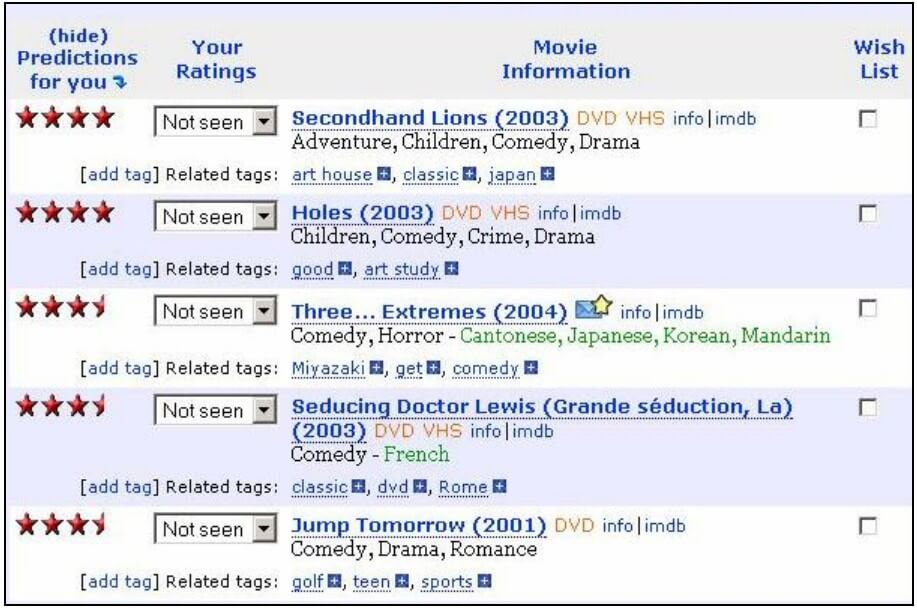
\includegraphics[width=0.9\textwidth]{images/2image2.jpeg}
\caption{MovieLens ใช้ระบบ Collaborative Filtering เพื่อทำนายว่าผู้ใช้งานรายนี้มีแนวโน้ม \cite{cfrs_nd}}
\label{fig:movielens}
\end{figure}

การให้คะแนน ผู้ใช้ระบุสถานะของหนัง เช่น "Not seen" คือยังไม่ได้ดู หรือให้คะแนน 1-5 ดาว การทำนายผล จากรูปภาพ ดังภาพที่ \ref{fig:movielens} ระบบสามารถทำนายได้ว่าผู้ใช้คนนี้มีแนวโน้มจะให้คะแนนหนังเรื่อง "Holes" ที่ 4 จาก 5 ดาว โดยคำนวณจากฐานข้อมูลความชอบของคนอื่นในระบบ ข้อมูลเสริม นอกจากคะแนนแล้ว ระบบยังมีการใช้แท็ก เช่น art house, classic และข้อมูลหมวดหมู่หนังเพื่อช่วยในการคัดกรอง         


\subsubsection{โครงสร้างของข้อมูล}

ในเชิงเทคนิค ข้อมูลเหล่านี้จะถูกมองเป็นความสัมพันธ์ระหว่าง 2 สิ่ง ได้แก่ ผู้ใช้ และ สิ่งของ โดยมีค่าคะแนน เป็นตัวเชื่อม และมักถูกนำมาจัดเรียงในรูปแบบของ เมทริกซ์ เพื่อใช้ในการประมวลผลอัลกอริทึมต่อไป \cite{cfrs_nd}             

\subsection{ระบบแนะนำตามเนื้อหา (Content-Based Recommendation Systems)}


\subsubsection{หลักการทำงานเบื้องต้น}

แม้ว่ารายละเอียดในแต่ละระบบจะแตกต่างกันออกไป แต่ระบบแนะนำตามเนื้อหาจะมีองค์ประกอบร่วมกัน 3 ประการคือ \cite{pazzani2007} 

\paragraph{วิธีการอธิบายคุณลักษณะของสิ่งของ ที่จะนำมาแนะนำ}

\paragraph{วิธีการสร้างโปรไฟล์ของผู้ใช้ เพื่อระบุประเภทของสิ่งที่ผู้ใช้ชอบ}

\paragraph{วิธีการเปรียบเทียบสิ่งของกับโปรไฟล์ผู้ใช้ เพื่อตัดสินใจว่าจะแนะนำอะไรให้}
โดยทั่วไป โปรไฟล์ของผู้ใช้จะถูกสร้างและอัปเดตโดยอัตโนมัติจากการตอบสนองหรือผลตอบรับ ของผู้ใช้ต่อสิ่งของที่ระบบเคยนำเสนอไปก่อนหน้า  


\subsubsection{การนำเสนอข้อมูลสิ่งของ (Item Representation)}

สิ่งของที่จะแนะนำมักถูกจัดเก็บไว้ในฐานข้อมูล ซึ่งข้อมูลเหล่านี้มีทั้งแบบ ข้อมูลที่มีโครงสร้าง และ ข้อมูลที่ไม่มีโครงสร้าง \cite{pazzani2007} 

\paragraph{ข้อมูลที่มีโครงสร้าง} เป็นข้อมูลที่มีจำนวนคุณลักษณะ (Attributes) ที่แน่นอน และแต่ละรายการจะถูกอธิบายด้วยชุดคุณลักษณะชุดเดียวกัน  ดังตัวอย่างตารางฐานข้อมูลร้านอาหารด้านล่าง ตารางที่ \ref{tab:exampleDBrestaurant}

\begin{table}[H]
\centering
\caption{ตัวอย่างฐานข้อมูลร้านอาหาร \cite{pazzani2007}}
\label{tab:exampleDBrestaurant}
\begin{tabular}{|c|l|l|l|l|}
\hline
\textbf{ID} & \textbf{Name} & \textbf{Cuisine} & \textbf{Service} & \textbf{Cost} \\
\hline
10001 & Mike's Pizza & Italian & Counter & Low \\ \hline
10002 & Chris's Cafe & French  & Table & Medium\\ \hline
10003 & Jacques Bistro  & French  & Table & High\\\hline
\end{tabular}
\end{table}

จากตารางนี้ ระบบสามารถเรียนรู้โปรไฟล์ผู้ใช้ได้ง่าย เช่น หากผู้ใช้ชอบร้านอาหารฝรั่งเศส 4 จาก 5 ร้าน ระบบจะระบุในโปรไฟล์ว่าผู้ใช้รายนี้มีความน่าจะเป็น 80\% ที่จะชอบร้านอาหารฝรั่งเศส

\paragraph{ข้อมูลที่ไม่มีโครงสร้าง} ข้อมูลประเภทนี้มักเป็นข้อความแบบอิสระ ซึ่งมีความซับซ้อนในการเรียนรู้โปรไฟล์มากกว่า ตัวอย่างที่เห็นได้ชัดคือ บทความข่าว ซึ่งเนื้อหาทั้งหมดจะถูกปฏิบัติเหมือนเป็นเขตข้อมูลข้อความขนาดใหญ่ที่ไม่จำกัดรูปแบบ ดังภาพที่ \ref{fig:newsarticle}

\begin{figure}[H]
\centering
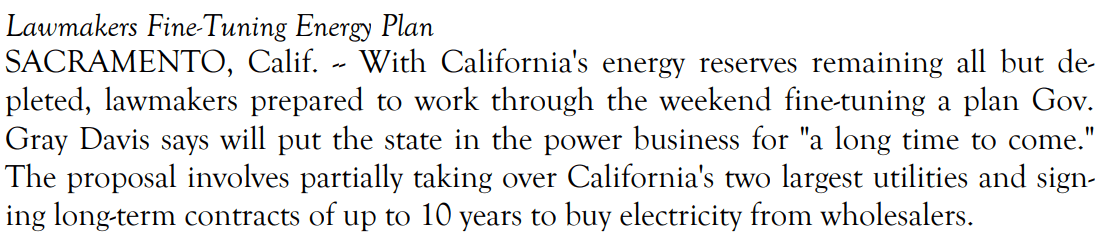
\includegraphics[width=0.9\textwidth]{images/2image3.png}
\caption{ส่วนหนึ่งของบทความหนังสือพิมพ์ \cite{pazzani2007}}
\label{fig:newsarticle}
\end{figure}

โดยปกติแล้ว เมื่อผู้ใช้โต้ตอบกับเว็บแอปพลิเคชัน ระบบจะแสดงรายการสิ่งของแบบสรุป เนื่องจากในฐานข้อมูลมีรายการจำนวนมากเกินกว่าจะแสดงบนหน้าเว็บได้หมด ระบบแนะนำตามเนื้อหาจึงต้องวิเคราะห์รายละเอียดของสิ่งของ เพื่อคัดเลือกชุดย่อยของรายการหรือจัดลำดับการแสดงผลให้ตรงกับความสนใจเฉพาะตัวของผู้ใช้มากที่สุด     

\subsection{ระบบแนะนำแบบผสมผสาน การสำรวจและการทดลอง (Hybrid Recommender Systems: Survey and Experiments)}


\subsubsection{บทนำและเทคนิคการแนะนำ}

งานวิจัยระบุว่าระบบแนะนำ กลายเป็นแอปพลิเคชันพื้นฐานในพาณิชย์อิเล็กทรอนิกส์ เพื่อช่วยผู้ใช้เลือกซื้อสินค้าหรือบริการท่ามกลางข้อมูลมหาศาล  โดยแบ่งเทคนิคหลักออกเป็น 5 ประเภท ดังตารางที่ \ref{tab:Recommendation techniques} \cite{hybrid_nd} 

\begin{table}[H]
\centering
\caption{เทคนิคการแนะนำ \cite{hybrid_nd}}
\label{tab:Recommendation techniques}
\begin{tabular}{|p{2.5cm}|p{3.8cm}|p{3.8cm}|p{4cm}|}
\hline
\textbf{เทคนิค} & \textbf{ข้อมูลพื้นหลัง} & \textbf{ข้อมูลนำเข้า} & \textbf{กระบวนการ} \\
\hline
Collaborative & การให้คะแนนของผู้ใช้คนอื่น & การให้คะแนนของผู้ใช้ปัจจุบัน & หาผู้ใช้ที่คล้ายกันและคาดการณ์จากคะแนนของพวกเขา \\ \hline
Content-based & คุณลักษณะของสินค้า & การให้คะแนนของผู้ใช้ต่อสินค้า & สร้างตัวจำแนก ที่ตรงกับพฤติกรรมผู้ใช้ \\ \hline
Demographic & ข้อมูลประชากรและการให้คะแนน & ข้อมูลประชากรของผู้ใช้ปัจจุบัน & หาผู้ใช้ที่มีลักษณะทางประชากรคล้ายกัน \\\hline
Utility-based & คุณลักษณะของสินค้า & ฟังก์ชันอรรถประโยชน์ (Utility function) & ใช้ฟังก์ชันคำนวณลำดับความสำคัญของสินค้า \\ \hline
Knowledge-based & คุณลักษณะของสินค้าและความรู้ & รายละเอียดความต้องการของผู้ใช้ & วิเคราะห์ความเชื่อมโยงระหว่างสินค้ากับความต้องการ \\\hline
\end{tabular}
\end{table}

Collaborative และ Content-based เป็นเทคนิคที่เน้นการเรียนรู้จากประวัติ เช่น ต้องรอให้คนไปรีวิวก่อนถึงจะทำงานได้ดี ส่วน Utility และ Knowledge ไม่ต้องรอประวัติการใช้งาน แต่ต้องมีข้อมูลสินค้าที่ชัดเจนและเงื่อนไขที่ผู้ใช้ระบุมาให้ ผู้วิจัยใช้ตารางนี้เป็นตัวตั้งต้นเพื่อชี้ให้เห็นว่า ไม่มีเทคนิคไหนสมบูรณ์แบบ เช่น Collaborative จะแนะนำของใหม่ที่ยังไม่มีใครรีวิวไม่ได้ จึงเป็นที่มาของการสร้าง ระบบไฮบริด


\subsubsection{ข้อดีและข้อเสียของแต่ละเทคนิค}

แต่ละเทคนิคมีจุดแข็งและจุดอ่อนต่างกัน เช่น ปัญหา Ramp-up คือปัญหาผู้ใช้ใหม่หรือสินค้าใหม่ที่ยังไม่มีคะแนนสะสม \cite{hybrid_nd} 

\begin{table}[H]
\centering
\caption{ข้อดีข้อเสียระหว่างเทคนิคการแนะนำต่าง ๆ \cite{hybrid_nd}}
\label{tab:Advantages and disadvantages of different counseling techniques}
\renewcommand{\arraystretch}{1.3}
\begin{tabular}{|p{2.5cm}|p{5.5cm}|p{5.5cm}|}
\hline
\textbf{เทคนิค} & \textbf{ข้อดี} & \textbf{ข้อเสีย} \\
\hline
Collaborative filtering (CF) &
(1) ไม่จำเป็นต้องมีข้อมูลคุณลักษณะของรายการ \gap
(2) สามารถค้นพบความสนใจแฝงของผู้ใช้ได้ &
(1) มีปัญหาผู้ใช้ใหม่และรายการใหม่ \gap
(2) ข้อมูลมักเบาบาง (sparsity) \gap
(3) ต้องการจำนวนผู้ใช้และคะแนนจำนวนมาก \\ \hline
Content-based (CN) &
(1) ให้คำแนะนำเฉพาะบุคคลได้ดี \gap
(2) ไม่พึ่งพาข้อมูลจากผู้ใช้คนอื่น &
(1) จำกัดอยู่ในขอบเขตความสนใจเดิมของผู้ใช้ \gap
(2) คุณภาพขึ้นกับคุณภาพของข้อมูลคุณลักษณะ \\ \hline
Demographic (DM) &
(1) เหมาะกับผู้ใช้ใหม่ \gap
(2) ไม่ต้องมีประวัติการให้คะแนนจำนวนมาก &
(1) ผู้ใช้ไม่อยากเปิดเผยข้อมูลส่วนตัว \gap
(2) การจัดกลุ่มอาจหยาบและไม่แม่นยำ \\ \hline
Utility-based (UT) &
(1) สามารถคำนึงถึงปัจจัยหลายด้าน เช่น ราคา เวลา ความสะดวก &
(1) ผู้ใช้ต้องให้ข้อมูลจำนวนมาก \gap
(2) การสร้างฟังก์ชันอรรถประโยชน์ทำได้ยาก \\ \hline
Knowledge-based (KB) &
(1) ไม่ประสบปัญหาผู้ใช้ใหม่หรือรายการใหม่ \gap
(2) เหมาะกับการตัดสินใจเชิงซับซ้อน &
(1) ต้องใช้ต้นทุนสูงในการสร้างและดูแลฐานความรู้ \gap
(2) ยากต่อการขยายระบบในระยะยาว \\ \hline
\end{tabular}
\end{table}

ตารางนี้แสดงให้เห็นว่าเทคนิคการแนะนำแต่ละแบบมีทั้งจุดเด่นและข้อจำกัดที่แตกต่างกัน โดย ไม่มีเทคนิคใดที่สามารถตอบโจทย์ได้ครบทุกด้าน เทคนิคอย่าง collaborative filtering มีจุดแข็งในการค้นหาความสนใจของผู้ใช้จากพฤติกรรมของผู้อื่น แต่ประสบปัญหาเมื่อข้อมูลมีจำนวนน้อย ขณะที่ content-based ให้คำแนะนำที่ตรงกับความสนใจส่วนบุคคลได้ดี แต่จำกัดอยู่ในกรอบความสนใจเดิมของผู้ใช้ ส่วนเทคนิคอย่าง knowledge-based สามารถให้คำแนะนำได้แม้ในกรณีที่ไม่มีข้อมูลประวัติ แต่ต้องแลกกับต้นทุนในการพัฒนาและดูแลระบบที่สูง 

จากการเปรียบเทียบดังกล่าว สะท้อนให้เห็นว่า การเลือกใช้เทคนิคเพียงวิธีเดียวอาจไม่เพียงพอ จึงเป็นที่มาของแนวคิดในการนำเทคนิคหลายแบบมาผสมผสานกัน เพื่อใช้จุดแข็งของแต่ละวิธีมาชดเชยข้อจำกัดซึ่งกันและกัน และนำไปสู่การพัฒนาระบบแนะนำแบบผสม 


\subsubsection{กลยุทธ์การผสมผสาน (Hybridization Strategies) 7 รูปแบบ} \cite{hybrid_nd}

\paragraph{Weighted}
นำคะแนนจากหลายเทคนิคมาคำนวณรวมกันโดยใช้น้ำหนักที่เหมาะสม

\paragraph{Switching}
ระบบจะเปลี่ยนเทคนิคการแนะนำโดยอัตโนมัติตามสถานการณ์ เช่น ถ้าไม่มีข้อมูลผู้ใช้จะใช้ Content-based แต่ถ้ามีข้อมูลมากพอจะสลับไปใช้ Collaborative

\paragraph{Mixed}
แสดงผลลัพธ์จากหลายเทคนิคพร้อมกันในรายการเดียว

\paragraph{Feature Combination}
นำคุณลักษณะจากแหล่งข้อมูลหนึ่งไปเสริมให้กับอีกเทคนิคหนึ่ง

\paragraph{Feature Augmentation}
ใช้ผลลัพธ์จากเทคนิคแรกเป็นข้อมูลนำเข้า ให้กับเทคนิคที่สอง

\paragraph{Cascade}
เทคนิคแรกจะทำการคัดกรองรายการเบื้องต้น และเทคนิคที่สองจะนำผลลัพธ์นั้นมาจัดลำดับ (Ranking) อีกครั้ง 

\paragraph{Meta-level}
นำโมเดลที่เรียนรู้จากเทคนิคหนึ่งไปใช้เป็นข้อมูลทั้งหมดให้อีกเทคนิคหนึ่งประมวลผลต่อ 


\subsubsection{กรณีศึกษา ระบบ Entree และ EntreeC}

Entree เป็นระบบแนะนำร้านอาหารที่พัฒนาขึ้นโดยใช้แนวคิดของ การแนะนำแบบอาศัยความรู้ ระบบจะใช้แบบจำลองความต้องการของผู้ใช้และความรู้เกี่ยวกับร้านอาหาร เช่น ประเภทอาหาร ราคา บรรยากาศ และสถานที่ เพื่อแนะนำร้านอาหารที่เหมาะสมที่สุด ผู้ใช้สามารถระบุเงื่อนไขต่าง ๆ เช่น ต้องการอาหารประเภทใด, ช่วงราคาที่เหมาะสม หรือลักษณะบรรยากาศของร้าน จากนั้นระบบจะใช้กฎเชิงความรู้ในการประเมินว่าร้านอาหารใดสอดคล้องกับความต้องการเหล่านั้นมากที่สุด สถาปัตยกรรมของระบบแสดงดังภาพที่ \ref{fig:entree} \cite{hybrid_nd} 

\begin{figure}[H]
\centering
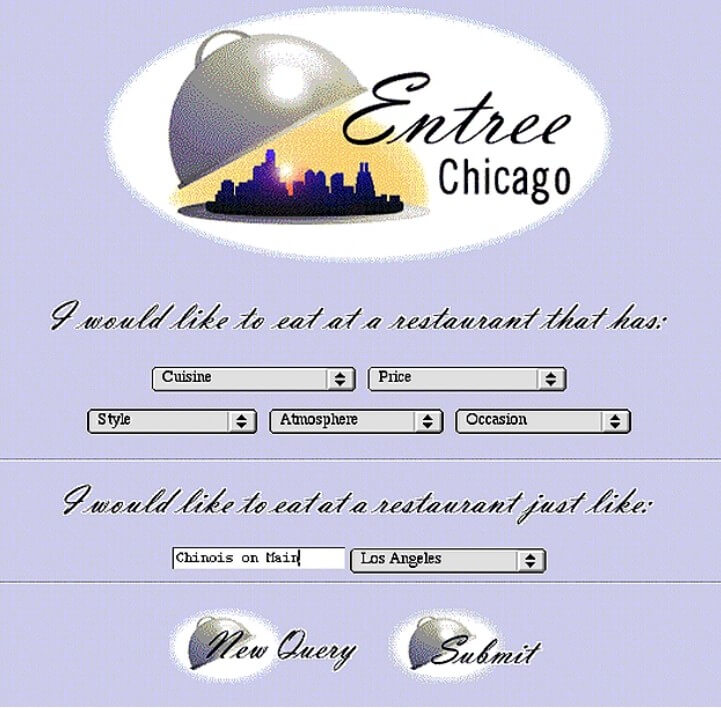
\includegraphics[width=0.9\textwidth]{images/2image4.jpeg}
\caption{สถาปัตยกรรมของระบบ Entree \cite{hybrid_nd}}
\label{fig:entree}
\end{figure}

EntreeC เป็นการพัฒนาต่อยอดจาก Entree โดยนำ collaborative filtering เข้ามาผสานกับระบบเดิม เป้าหมายคือการเพิ่มประสิทธิภาพของคำแนะนำโดยอาศัยทั้งความรู้เชิง Domain และประสบการณ์จากผู้ใช้คนอื่น โครงสร้างของ EntreeC ประกอบด้วย 2 ส่วนหลัก ได้แก่ ระบบแนะนำแบบอาศัยความรู้ (knowledge-based component) และระบบ collaborative filtering ในส่วนของ knowledge-based จะสร้างคะแนนเชิงความหมาย (semantic ratings) สำหรับร้านอาหารแต่ละแห่ง จากนั้นคะแนนเหล่านี้จะถูกนำไปใช้เป็นข้อมูลนำเข้าให้กับ collaborative filtering เพื่อปรับปรุงการทำนายความชอบของผู้ใช้ แสดงดังภาพที่ \ref{fig:entreec} 

\begin{figure}[H]
\centering
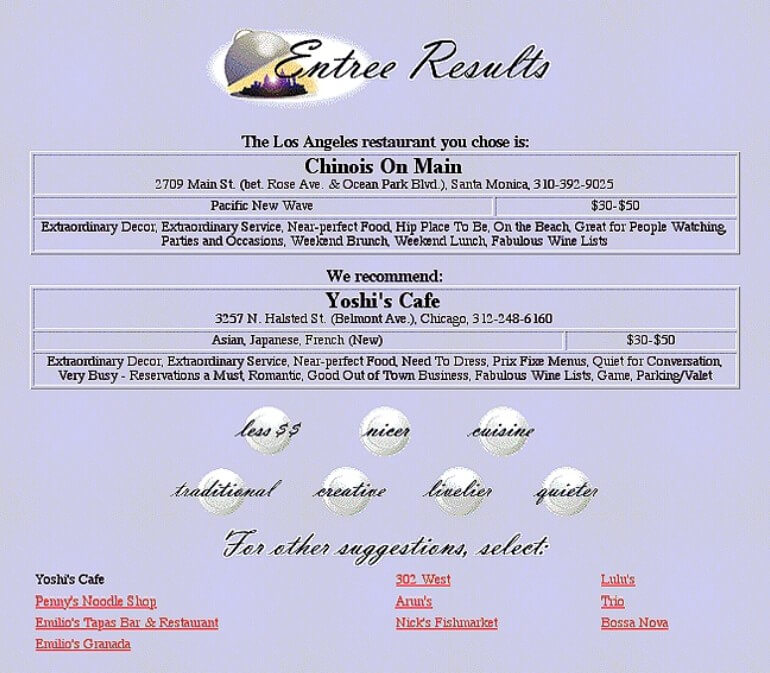
\includegraphics[width=0.9\textwidth]{images/2image5.jpeg}
\caption{สถาปัตยกรรมของระบบ EntreeC \cite{hybrid_nd}}
\label{fig:entreec}
\end{figure}



\subsubsection{การทดลอง}

การทดลองมีเป้าหมายเพื่อประเมินว่า การผสมผสานคะแนนเชิงความหมายจากระบบ knowledge-based เข้ากับ collaborative filtering จะช่วยเพิ่มคุณภาพของคำแนะนำหรือไม่ โดยเปรียบเทียบผลลัพธ์ระหว่าง ระบบ collaborative filtering แบบดั้งเดิม กับระบบ EntreeC ที่ใช้คะแนนเชิงความหมายร่วมด้วย \cite{hybrid_nd}

โดยวิธีทดลองคือผู้ใช้จะถูกขอให้ให้คะแนนร้านอาหารในระบบ จากนั้นคะแนนเหล่านี้จะถูกใช้สร้างแบบจำลอง collaborative filtering สองรูปแบบ ได้แก่แบบใช้เฉพาะคะแนนจริงจากผู้ใช้ และแบบใช้คะแนนจริงรวมกับคะแนนเชิงความหมายจากระบบ Entree ผลลัพธ์ของทั้งสองแบบจะถูกนำมาเปรียบเทียบโดยใช้ตัวชี้วัดมาตรฐาน เช่น ความแม่นยำในการทำนาย (prediction accuracy) โดยสูตรที่ใช้จะมีดังนี้ 

\vspace{1em}
\paragraph{สูตร Cosine Similarity}

\begin{equation}
\cos(A,B)=
\frac{\sum_{i=1}^{n} V_{A,i}V_{B,i}}
{\sqrt{\sum_{i=1}^{n}V_{A,i}^{2}}
 \sqrt{\sum_{i=1}^{n}V_{B,i}^{2}}}
\label{eq:cosine}
\end{equation}

\noindent โดยที่

\noindent
\begin{tabular}{@{}l @{\ :\ } p{0.85\textwidth}}
$\cos(A,B)$ & ค่าความคล้ายคลึงระหว่างข้อมูลสองชุด $A$ และ $B$ มีค่าอยู่ระหว่าง 0 ถึง 1 กรณีที่เวกเตอร์ไม่มีค่าติดลบ หมายความว่า ยิ่งใกล้ 1 ยิ่งคล้ายกันมาก ยิ่งใกล้ 0 ยิ่งต่างกันมาก \\
$A, B$ & ข้อมูลสองชุดที่ต้องการเปรียบเทียบ เช่น ผู้ใช้สองคน หรือรายการสองรายการ \\
$V_A, V_B$ & เวกเตอร์ที่แทนข้อมูลของ $A$ และ $B$ เช่น เวกเตอร์พฤติกรรมหรือเวกเตอร์คะแนน \\
$V_{A,i}, V_{B,i}$ & ค่าในตำแหน่งที่ $i$ ของเวกเตอร์ $V_A$ และ $V_B$ ตามลำดับ \\
$i$ & ตัวนับตำแหน่งของค่าในเวกเตอร์ เริ่มจาก $1$ ถึง $n$ \\
$n$ & จำนวนค่าทั้งหมดในเวกเตอร์ (จำนวนมิติ) \\
$\sum_{i=1}^{n}$ & เครื่องหมายผลรวม คือการบวกค่าตั้งแต่ตำแหน่งที่ $1$ ถึง $n$ \\
\end{tabular}

\bigskip
\noindent ส่วนประกอบของสูตร

\noindent
\begin{tabular}{@{}l @{\ :\ } p{0.85\textwidth}}
ตัวเศษ & $\sum_{i=1}^{n} V_{A,i}V_{B,i}$ คือผลคูณจุด (dot product) นำค่าในตำแหน่งเดียวกันของ $V_A$ และ $V_B$ มาคูณกัน แล้วบวกรวมทั้งหมด ยิ่งค่าตำแหน่งเดียวกันมีขนาดใหญ่ทั้งคู่ ผลรวมยิ่งมาก \\
ตัวส่วน & $\sqrt{\sum V_{A,i}^{2}}\sqrt{\sum V_{B,i}^{2}}$ คือผลคูณของความยาวเวกเตอร์ $\lVert V_A \rVert \cdot \lVert V_B \rVert$ ใช้ปรับสเกลให้เปรียบเทียบเฉพาะ ``ทิศทาง'' โดยไม่ขึ้นกับขนาดของข้อมูล \\
\end{tabular}

\bigskip
\noindent ตัวอย่างการคำนวณ

\noindent กำหนด $V_A = (1, 2, 3)$ และ $V_B = (2, 1, 0)$

\begin{align*}
\text{ตัวเศษ} &= (1)(2) + (2)(1) + (3)(0) = 4 \\
\lVert V_A \rVert &= \sqrt{1^2 + 2^2 + 3^2} = \sqrt{14} \approx 3.742 \\
\lVert V_B \rVert &= \sqrt{2^2 + 1^2 + 0^2} = \sqrt{5} \approx 2.236 \\
\cos(A,B) &= \frac{4}{3.742 \times 2.236} \approx 0.478
\end{align*}

\noindent แปลผล: ค่าเท่ากับ $0.478$ แสดงว่า $A$ และ $B$ มีความคล้ายกันในระดับปานกลาง
สูตรนี้ใช้วัดความคล้ายกันของเวกเตอร์ ซึ่งในบริบทของงานวิจัยคือ เวกเตอร์แทนพฤติกรรมหรือการให้คะแนนของผู้ใช้หรือเวกเตอร์แทนคุณลักษณะของร้านอาหาร ถ้าค่า cos(A,B) ใกล้ 1 แสดงว่าสองเวกเตอร์มีทิศทางคล้ายกันมาก ซึ่งหมายถึง เวกเตอร์ทั้งสองมีลักษณะคล้ายกัน \cite{hybrid_nd}

\vspace{1em}
\paragraph{สูตรความคล้ายเชิงความหมายของการให้คะแนน (Heuristic similarity)}
ในงานวิจัย ผู้เขียนไม่ได้ดูแค่ตัวเลขคะแนน แต่ดู ``ความหมาย'' ของการกระทำ
เช่น Browse, Cheaper, Nicer, Trad, Creative เป็นต้น
จึงสร้างตารางความคล้ายของการให้คะแนน
แล้วนิยามฟังก์ชันระยะห่างของการกระทำเป็น

\[
d(a,b)
\]

\noindent จากนั้นนิยามความคล้ายของเวกเตอร์ $A$ และ $B$ เป็น

\begin{equation}
h(A,B)=\frac{\sum_{(a,b)\in R} d(a,b)}{|R|}
\label{eq:h}
\end{equation}

\noindent โดยที่

\noindent
\begin{tabular}{@{}l @{\ :\ } p{0.85\textwidth}}
$h(A,B)$ & ค่าความคล้ายแบบ Heuristic ระหว่างผู้ใช้ $A$ และ $B$ คำนวณจากค่าเฉลี่ยของ $d(a,b)$ ของทุกรายการที่ทั้งสองคนให้คะแนนร่วมกัน \\
$A, B$ & ผู้ใช้สองคนที่ต้องการวัดความคล้ายคลึง โดยแต่ละคนแทนด้วยเวกเตอร์การให้คะแนนของตนเอง \\
$R$ & เซตร้านอาหารที่ผู้ใช้ $A$ และ $B$ ให้คะแนนร่วมกัน ซึ่งนำมาเปรียบเทียบได้เฉพาะร้านที่ทั้งคู่เคยให้คะแนน \\
$|R|$ & จำนวนร้านอาหารในเซต $R$ ใช้เป็นตัวหารเพื่อหาค่าเฉลี่ย \\
$a \in R_A$ & การให้คะแนนหรือพฤติกรรมของผู้ใช้ $A$ ที่มีต่อร้านหนึ่งร้าน เช่น Browse, Cheaper, Nicer \\
$b \in R_B$ & การให้คะแนนหรือพฤติกรรมของผู้ใช้ $B$ ที่มีต่อร้านเดียวกันกับ $a$ \\
$d(a,b)$ & ค่าความคล้ายเชิงความหมายระหว่างการกระทำ $a$ และ $b$ ที่อ่านจากตารางความคล้ายที่ผู้เขียนสร้างไว้ หมายความว่าถ้าความหมายใกล้กัน ค่ายิ่งสูง \\
$\sum_{(a,b)\in R}$ & ผลรวมของ $d(a,b)$ ทุกคู่การให้คะแนนในร้านที่ทั้งสองคนให้ร่วมกัน \\
\end{tabular}

\bigskip

\noindent ขั้นตอนคือ (1) หาร้านที่ผู้ใช้ทั้งสองให้คะแนนตรงกัน (2) แต่ละร้าน เปิดตารางดูว่าการกระทำของ $A$ กับ $B$ มีความหมายใกล้กันแค่ไหน ได้เป็น $d(a,b)$ (3) นำค่าทุกร้านมาบวกกัน แล้วหารด้วยจำนวนร้าน $|R|$ ได้ค่าเฉลี่ยเป็น $h(A,B)$ สูตรนี้ใช้วัดว่าเวกเตอร์ “คล้ายกันแค่ไหนในเชิงความหมายของการให้คะแนน” ไม่ใช่แค่ดูว่าคะแนนเท่ากันหรือไม่ แต่ดูว่าความรู้สึกของคะแนนใกล้กันแค่ไหน เช่น “Lively” กับ “Quiet” ถือว่าเป็นตรงข้าม หรือ “Traditional” กับ “Creative” ก็เป็นอีกคู่ตรงข้าม นี่คือจุดเด่นของ EntreeC ที่ต่างจาก collaborative filtering ปกติ \cite{hybrid_nd}

\vspace{1em}
\paragraph{สูตรสัมประสิทธิ์สหสัมพันธ์เพียร์สัน (Pearson Correlation Coefficient)}
สูตรนี้ใช้วัดว่าผู้ใช้สองคนให้คะแนนไปในทิศทางเดียวกันมากน้อยแค่ไหน โดยดูเฉพาะร้านที่ทั้งคู่ให้คะแนนร่วมกัน

\begin{equation}
r(A,B)=
\frac{n\sum R_A R_B-\left(\sum R_A\right)\left(\sum R_B\right)}
{\sqrt{\left(n\sum R_A^2-\left(\sum R_A\right)^2\right)
\left(n\sum R_B^2-\left(\sum R_B\right)^2\right)}}
\label{eq:pearson}
\end{equation}

\noindent โดยที่

\noindent
\begin{tabular}{@{}l @{\ :\ } p{0.85\textwidth}}
$r(A,B)$ & ค่าสัมประสิทธิ์สหสัมพันธ์เพียร์สันระหว่างผู้ใช้ $A$ และ $B$ บอกว่าการให้คะแนนของทั้งสองคนสัมพันธ์กันแค่ไหน มีค่าอยู่ระหว่าง $-1$ ถึง $1$ \\
$A, B$ & ผู้ใช้สองคนที่ต้องการเปรียบเทียบ โดยแต่ละคนแทนด้วยเวกเตอร์คะแนนที่ตนเองให้ร้านอาหาร \\
$R_A$ & คะแนนที่ผู้ใช้ $A$ ให้ร้านอาหารแต่ละร้าน เฉพาะร้านที่ทั้งคู่ให้คะแนนร่วมกัน \\
$R_B$ & คะแนนที่ผู้ใช้ $B$ ให้ร้านอาหารแต่ละร้าน เฉพาะร้านที่ทั้งคู่ให้คะแนนร่วมกัน \\
$n$ & จำนวนร้านอาหารที่ผู้ใช้ $A$ และ $B$ ให้คะแนนร่วมกัน \\
$\sum R_A R_B$ & นำคะแนนของ $A$ และ $B$ ในร้านเดียวกันมาคูณกัน แล้วบวกรวมทุกร้าน \\
$\sum R_A,\ \sum R_B$ & ผลรวมคะแนนทั้งหมดที่ $A$ และ $B$ ให้ตามลำดับ \\
$\sum R_A^2,\ \sum R_B^2$ & นำคะแนนแต่ละร้านของ $A$ หรือ $B$ มายกกำลังสอง แล้วบวกรวมทุกร้าน \\
\end{tabular}

\bigskip
\noindent ส่วนประกอบของสูตร

\medskip
\noindent
\begin{tabular}{@{}l @{\ :\ } p{0.85\textwidth}}
ตัวเศษ & $n\sum R_A R_B-\left(\sum R_A\right)\left(\sum R_B\right)$ วัดว่าคะแนนของ $A$ และ $B$ ``ขึ้นลงไปด้วยกัน'' หรือไม่ ถ้าร้านที่ $A$ ให้สูง $B$ ก็ให้สูงด้วย ค่าจะเป็นบวก ถ้าตรงข้ามกันค่าจะเป็นลบ \\[1.5em]
ตัวส่วน & $\sqrt{\left(n\sum R_A^2-\left(\sum R_A\right)^2\right)\left(n\sum R_B^2-\left(\sum R_B\right)^2\right)}$ วัดการกระจายของคะแนนแต่ละคน ใช้ปรับสเกลให้ผลลัพธ์อยู่ระหว่าง $-1$ ถึง $1$ เสมอ \\
\end{tabular}

\noindent การแปลผลค่า $r(A,B)$

\noindent
\begin{tabular}{@{}l @{\ :\ } p{0.85\textwidth}}
ใกล้ $1$ & ผู้ใช้ทั้งสองชอบคล้ายกันมาก ร้านที่คนหนึ่งให้สูง อีกคนก็ให้สูง \\
ใกล้ $0$ & การให้คะแนนของทั้งสองคนไม่เกี่ยวข้องกัน \\
ใกล้ $-1$ & ผู้ใช้ทั้งสองชอบตรงข้ามกัน ร้านที่คนหนึ่งให้สูง อีกคนให้ต่ำ \\
\end{tabular}

\bigskip
\noindent ตัวอย่างการคำนวณ

\noindent กำหนดให้ผู้ใช้ $A$ และ $B$ ให้คะแนนร้านอาหารร่วมกัน 3 ร้าน คือ $R_A = (5, 3, 1)$ และ $R_B = (4, 3, 2)$

\begin{align*}
n &= 3 \\
\sum R_A &= 9, \quad \sum R_B = 9 \\
\sum R_A R_B &= 20 + 9 + 2 = 31 \\
\sum R_A^2 &= 35, \quad \sum R_B^2 = 29 \\
r(A,B) &= \frac{3(31)-(9)(9)}{\sqrt{\left(3(35)-81\right)\left(3(29)-81\right)}}
= \frac{12}{\sqrt{24 \times 6}} = \frac{12}{12} = 1
\end{align*}

\noindent แปลผล: ค่าเท่ากับ $1$ แสดงว่า $A$ และ $B$ ให้คะแนนไปในทิศทางเดียวกันอย่างสมบูรณ์

นักวิจัยใช้สูตรนี้เป็นแกนหลักของ collaborative filtering หลังจากที่แปลงพฤติกรรมผู้ใช้ให้เป็นเวกเตอร์คะแนนแล้ว ตัวอย่างหน้าจอเมนูหลักของระบบแสดงดังภาพที่ \ref{fig:menu} \cite{hybrid_nd}

\begin{figure}[H]
\centering
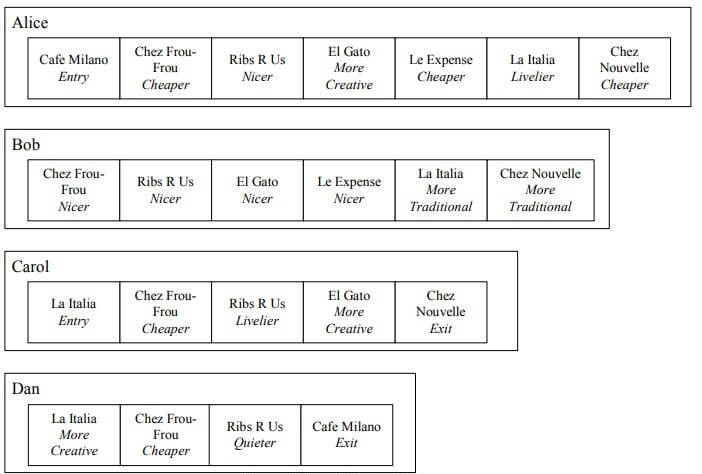
\includegraphics[width=0.9\textwidth]{images/2image6.jpeg}
\caption{ตัวอย่างการนำเสนอเมนูหลัก \cite{hybrid_nd}}
\label{fig:menu}
\end{figure}

\noindent ได้ผลการทดลอง ดังนี้

\begin{table}[H]
\centering
\caption{การคำนวณความคล้ายโดยใช้สหสัมพันธ์ \cite{hybrid_nd}}
\label{tab: Calculating similarity using correlation}
\begin{tabular}{|c|l|}
\hline
\textbf{User} & \textbf{Correlation} \\
\hline
Bob & 1.00  \\ \hline
Carol & 0.08  \\ \hline
Dan & 0.70  \\ \hline
\end{tabular}
\end{table}

ตารางที่ \ref{tab: Calculating similarity using correlation} แสดงผลการคำนวณ ความคล้ายของผู้ใช้ โดยใช้สูตร Pearson Correlation จากคะแนนที่ผู้ใช้ให้กับร้านอาหาร บ่งบอกว่าเวกเตอร์มีรสนิยมคล้ายกันมากแค่ไหน โดยค่าใกล้ 1 คือชอบเหมือนกันมาก ค่าใกล้ 0 คือไม่เกี่ยวข้องกัน ค่าใกล้ -1 คือชอบตรงข้ามกัน 

\begin{table}[H]
\centering
\caption{การคำนวณความคล้ายโดยใช้โคไซน์ \cite{hybrid_nd}}
\label{tab: Calculating similarity using cosine}
\begin{tabular}{|c|l|}
\hline
\textbf{User} & \textbf{Cosine} \\
\hline
Bob & 0.024  \\ \hline
Carol & 0.057  \\ \hline
Dan & 0.036  \\ \hline
\end{tabular}
\end{table}

ตารางที่ \ref{tab: Calculating similarity using cosine} แสดงการคำนวณ ความคล้ายของเวกเตอร์พฤติกรรมผู้ใช้ โดยใช้สูตร cosine similarity เปรียบเทียบผู้ใช้จาก “รูปแบบพฤติกรรม” ไม่ใช่จากค่าเฉลี่ยคะแนนและใช้เป็นอีกแนวทางหนึ่งของ collaborative filtering โดยค่าใกล้ 1 คือรูปแบบพฤติกรรมคล้ายกันมาก ค่าใกล้ 0 คือไม่คล้ายกัน ค่าใกล้ -1 คือตรงข้ามกัน 

\begin{table}[H]
\centering
\caption{ระยะห่างเชิง Heuristic แบบเฉพาะที่และแบบภาพรวม \cite{hybrid_nd}}
\label{tab: Calculating similarity using heuristic}
\resizebox{\textwidth}{!}{%
\begin{tabular}{|c|c|c|c|c|c|c|c|c|}
\hline
\textbf{} & \textbf{Cafe Milano} & \textbf{Chez FrouFrou} & \textbf{Chez Nouvelle } & \textbf{El Gato} & \textbf{La Italia} & \textbf{Le Expense} & \textbf{Ribs R Us} & \textbf{Average distance} \\
\hline
Bob & 0  & -1 & -0.5 & 0.5 & -0.5 & -1 & 1 & -0.21 \\ \hline
Carol & 0  & -1 & 0 & 1 & 0 & 0 & -0.5 & -0.07 \\ \hline
Dan & 1  & 1 & 0 & 0 & 0.5 & 0 & 0.5 & 0.43 \\ \hline
\end{tabular}%
}
\end{table}

ตารางที่ \ref{tab: Calculating similarity using heuristic} เป็นวิธีใหม่ที่ผู้วิจัยเสนอ คือการวัดความคล้ายของเวกเตอร์จากความหมายของพฤติกรรม (semantic similarity) แต่ละช่องในตารางคำนวณจากสูตร Local Heuristic Distance $d(a,b)$ ซึ่งวัดระยะห่างเชิงความหมายของการกระทำทีละร้านระหว่างเวกเตอร์ทั้งสอง ส่วนคอลัมน์สุดท้าย (Average distance) คือ Global Heuristic Distance $h(A,B) = \frac{\sum d(a,b)}{|R|}$ ซึ่งนำค่า local distance มารวมกันทุก ๆ ร้านที่เวกเตอร์ให้คะแนนร่วมกันเพื่อวัดว่าโดยรวมแล้ว เวกเตอร์คล้ายกันแค่ไหนในเชิงพฤติกรรมและความรู้สึก พิสูจน์ว่าการดูความหมายของคะแนน ให้ผลดีกว่าการดูแค่ตัวเลข และเป็นเหตุผลสำคัญที่ระบบ EntreeC ให้ผลลัพธ์ดีกว่า collaborative filtering แบบเดิม 

ผลการทดลองแสดงให้เห็นว่า ระบบ EntreeC ซึ่งใช้คะแนนเชิงความหมายร่วมกับ collaborative filtering ให้ผลลัพธ์ที่ดีกว่าระบบ collaborative filtering แบบดั้งเดิมอย่างชัดเจน โดยเฉพาะในกรณีที่ข้อมูลการให้คะแนนของผู้ใช้ยังมีจำนวนน้อย ระบบสามารถลดปัญหา sparsity และ ramp-up ได้อย่างมีประสิทธิภาพ ส่งผลให้คำแนะนำมีความแม่นยำมากขึ้นตั้งแต่ระยะแรกของการใช้งาน 

\subsection{การเรียนรู้ของเครื่องจักร (Machine Learning for RS)}

เนื้อหาในงานวิจัย Toward the next generation of recommender systems: a survey of the state-of-the-art and possible extensions อธิบายถึงการนำเทคนิคการเรียนรู้ของเครื่องจักร (Machine Learning - ML) และเทคโนโลยีทางสถิติมาประยุกต์ใช้เพื่อประมาณค่าความพึงพอใจ (Rating Estimation) ของผู้ใช้อย่างกว้างขวาง โดยแบ่งออกเป็นกลุ่มหลัก ๆ ดังนี้ \cite{nextgen_nd} 


\subsubsection{การเรียนรู้ในระบบ Content-based}

ระบบนี้ใช้ ML เพื่อสร้างโมเดลที่เรียนรู้ความชอบของผู้ใช้จากลักษณะของไอเทมที่เคยชอบในอดีต ได้แก่ \cite{nextgen_nd} 

\paragraph{Naive Bayes Classifier}
ใช้ประเมินความน่าจะเป็นที่ผู้ใช้จะชอบเอกสารหรือเว็บไซต์ โดยคำนวณจากคำสำคัญ ที่ปรากฏ 

\paragraph{Winnow Algorithm}
ระบุว่าเป็นอัลกอริทึมที่มีประสิทธิภาพสูงในสถานการณ์ที่มีฟีเจอร์หรือลักษณะของข้อมูลจำนวนมาก 

\paragraph{เทคนิคอื่น ๆ}
มีการกล่าวถึงการใช้ Decision Trees, Artificial Neural Networks และ Clustering เพื่อสร้างแบบจำลองการทำนายความชอบจากข้อมูลเนื้อหา 


\subsubsection{การเรียนรู้ในระบบ Collaborative Filtering}

งานวิจัยจำแนกแนวทางที่ใช้ ML เป็นกลุ่ม Model-based algorithms ซึ่งจะเรียนรู้โมเดลจากชุดข้อมูลการให้คะแนนเพื่อนำไปทำนายในอนาคต ได้แก่ \cite{nextgen_nd}

\paragraph{โมเดลเชิงความน่าจะเป็น (Probabilistic Models)}
เช่น Cluster models ที่จัดกลุ่มผู้ใช้ที่มีลักษณะคล้ายกัน และ Bayesian Networks ที่มองว่าไอเทมแต่ละชิ้นเป็นโหนดในเครือข่ายเพื่อหาความสัมพันธ์ในการให้คะแนน 

\paragraph{การลดมิติข้อมูล (Dimensionality Reduction)}
มีการใช้เทคนิค Singular Value Decomposition (SVD) เพื่อจัดการกับปัญหาข้อมูลที่เบาบาง โดยการย่อยเมทริกซ์การให้คะแนนให้เหลือมิติที่สำคัญ 

\paragraph{Advanced ML Models}
มีการพูดถึงการใช้ Regression, Maximum Entropy, และ Markov Decision Processes (MDP) สำหรับมองการแนะนำเป็นปัญหาการตัดสินใจเชิงลำดับ 

\paragraph{Latent Semantic Models}
เช่น Probabilistic Latent Semantic Analysis (pLSA) และ Latent Dirichlet Allocation (LDA) เพื่อหาหัวข้อหรือลักษณะที่ซ่อนอยู่ (Latent variables) ของผู้ใช้และไอเทม 


\subsubsection{การเรียนรู้สำหรับการพัฒนาในอนาคต}

งานวิจัยยังเสนอให้นำเทคนิค ML ขั้นสูงมาใช้เพื่อก้าวข้ามขีดจำกัดเดิม ได้แก่ \cite{nextgen_nd}

\paragraph{Active Learning}
เสนอนำมาใช้เพื่อเลือกชุดข้อมูลฝึกฝนอย่างมีประสิทธิภาพ เพื่อให้ระบบเรียนรู้โปรไฟล์ผู้ใช้ได้เร็วขึ้นโดยรบกวนผู้ใช้น้อยที่สุด 

\paragraph{Hierarchical Bayesian Methods}
ใช้สำหรับระบบแนะนำแบบหลายมิติ (Multidimensional) เพื่อคำนวณความสัมพันธ์ระหว่างผู้ใช้ ไอเทม และบริบท เช่น เวลาหรือสถานที่ 

% -----------------------------------------------------------
\section{งานวิจัยและทฤษฎีเฉพาะด้านระบบแนะนำแบบหลายพฤติกรรม (Multi-Behavior Recommendation Systems - MBRS)}
% -----------------------------------------------------------

ระบบแนะนำแบบหลายพฤติกรรมเป็นแนวคิดที่ก้าวหน้ากว่าระบบเดิม โดยมุ่งเป้าไปที่การใช้พฤติกรรมของผู้ใช้หลายรูปแบบมาเรียงต่อกันเป็นห่วงโซ่ เช่น การคลิกอ่านเนื้อหา, การเพิ่มลงตะกร้า และการเช่า เพื่อทำนายพฤติกรรมเป้าหมายสุดท้ายในห่วงโซ่ ซึ่งสามารถแก้ปัญหา Data Sparsity ได้อย่างมีประสิทธิภาพ โดยในโครงงานนี้ได้ออกแบบห่วงโซ่พฤติกรรมไว้เป็น View $\rightarrow$ Cart $\rightarrow$ Rent โดยมีการเช่าเป็นพฤติกรรมเป้าหมายหลัก ทั้งนี้พฤติกรรมการคลิกอ่านเนื้อหา จะถูกรวบรวมจากพฤติกรรมจริงของผู้ใช้ภายในเว็บแอปพลิเคชัน เพื่อนำไปใช้ฝึกโมเดลรอง รายละเอียดแสดงในบทที่ 3

\subsection{Neural Multi-Task Recommendation (NMTR)}

โมเดล NMTR ที่มองการทำนายพฤติกรรมต่างๆ เป็นงานหลายงานที่เกี่ยวข้องกัน (Multi-Task Learning) โดยออกแบบให้โมเดลมีการแชร์ชั้นข้อมูล และส่งต่อผลลัพธ์แบบลำดับขั้น งานวิจัยนี้พิสูจน์ให้เห็นว่า แม้ข้อมูลพฤติกรรมหลักจะมีน้อย แต่การนำข้อมูลพฤติกรรมรอง เช่น การกดดูสินค้า มาช่วยฝึกสอนโมเดล ก็สามารถเพิ่มความแม่นยำในการทำนายได้อย่างมีนัยสำคัญ \cite{gao2019} 


\subsubsection{พฤติกรรมเป้าหมาย}
พฤติกรรมเป้าหมาย หมายถึงพฤติกรรมที่เป็นจุดประสงค์สูงสุดของระบบหรือสร้างรายได้โดยตรง เช่น การซื้อ หรือการเช่า ซึ่งโดยธรรมชาติแล้วข้อมูลส่วนนี้มักจะมีปริมาณน้อยและกระจายตัวสูง

\subsubsection{พฤติกรรมช่วยตัดสินใจ}
พฤติกรรมช่วยตัดสินใจ คือพฤติกรรมย่อยที่เกิดขึ้นในระหว่างเส้นทางการตัดสินใจของผู้ใช้ ซึ่งมีปริมาณข้อมูลที่หนาแน่นกว่าและสามารถนำมาใช้เป็นสัญญาณบ่งชี้ความสนใจแฝงได้ แบ่งออกเป็น การแสดงออกที่ชัดเจนและตรงไปตรงมาและพฤติกรรมที่แฝงนัยความสนใจซึ่งต้องอาศัยการตีความ

\subsection{Graph Neural Networks for Multi-Behavior (MBGCN)}

อีกแนวทางหนึ่งคือการใช้โครงสร้างกราฟเข้ามาช่วย โดยจำลองความสัมพันธ์ของผู้ใช้ สินค้า และการกระทำต่างๆ ให้อยู่ในรูปแบบของโหนดและเส้นเชื่อม จุดเด่นของ MBGCN คือกระบวนการแพร่กระจายข้อมูลภายในกราฟ ที่ช่วยให้ระบบเข้าใจถึงอิทธิพลและลำดับความสำคัญของแต่ละพฤติกรรมที่มีผลต่อการตัดสินใจซื้อได้ลึกซึ้งกว่าโมเดลทั่วไป \cite{mbgcn_nd} 

\subsubsection{การแชร์พารามิเตอร์ร่วมกัน}
เสนอหลักการว่า ไม่ว่าผู้ใช้จะกระทำพฤติกรรมใด เช่น ดู หรือซื้อ บุคลิกภาพและความชอบพื้นฐานของผู้ใช้คนนั้น (User Embedding) ควรจะเป็นชุดข้อมูลเดียวกันที่ถูกแชร์ร่วมกันในทุกงาน

\subsubsection{การทำนายแบบลดหลั่นตามลำดับ}
โมเดลถูกออกแบบให้มีการส่งต่อผลลัพธ์การทำนายเป็นทอด ๆ ตามลำดับขั้นของ โดยอาศัยสมมติฐานว่าผู้ใช้มักจะต้องผ่านพฤติกรรมขั้นต้นก่อนจึงจะไปสู่ขั้นต่อไปได้ ซึ่งช่วยให้ข้อมูลจากพฤติกรรมต้นน้ำช่วยกรองความสนใจให้แม่นยำขึ้น

\subsection{Contrastive Meta-Learning for Multi-Behavior (CML)}

เสนอกรอบการทำงานที่ผสมผสานระหว่าง Contrastive Learning เพื่อแยกแยะความต่างของพฤติกรรม และ Meta-Learning เพื่อช่วยให้โมเดลปรับตัวเข้ากับความชอบเฉพาะบุคคลได้อย่างรวดเร็ว แนวทางนี้มีประโยชน์อย่างมากในการแก้ปัญหาข้อมูลเบาบาง โดยเฉพาะในกรณีที่ผู้ใช้มีประวัติการใช้งานน้อย ระบบก็ยังสามารถจับทิศทางความสนใจได้ \cite{wei2022} 

  
\subsubsection{การแพร่กระจายข้อมูลแบบตระหนักถึงพฤติกรรม}
ในกราฟที่เชื่อมโยงระหว่างผู้ใช้และสินค้า โมเดลมีความสามารถในการเรียนรู้น้ำหนักความสำคัญของแต่ละพฤติกรรมได้โดยอัตโนมัติ เพื่อแยกแยะว่าพฤติกรรมใด ส่งผลต่อความชอบของผู้ใช้มากน้อยเพียงใด

  
\subsubsection{การเรียนรู้ความหมายเชิงพฤติกรรม}
มีการสร้างกราฟความสัมพันธ์ระหว่างสินค้า (Item-Item Graph) เพื่อเรียนรู้ว่าสินค้าใดบ้างที่มักถูกกระทำด้วยพฤติกรรมเดียวกัน เช่น สินค้า A และ B มักถูกซื้อพร้อมกัน ทำให้โมเดลเข้าใจบริบทของสินค้าได้ลึกซึ้งขึ้น

\subsection{Knowledge-Enhanced Contrastive Learning (KCL)}

สำหรับกรณีที่ข้อมูลพฤติกรรมมีจำกัด งานวิจัย KMCLR ได้เสนอให้นำกราฟความรู้มาใช้เสริมความเข้าใจในตัวสินค้า ควบคู่กับเทคนิค Contrastive Learning เพื่อเชื่อมโยงความสัมพันธ์ระหว่างพฤติกรรม เช่น การดูและการซื้อ วิธีนี้ช่วยให้ระบบสามารถดึงข้อมูลเชิงลึกมาใช้ประโยชน์ ทำให้การแนะนำมีความแม่นยำแม้จะเป็นสินค้าใหม่หรือผู้ใช้ใหม่ก็ตาม \cite{xuan2023} 

\subsection{Graph Heterogeneous Multi-Relational Recommendation}

งานวิจัยนี้เสนอแนวทางใหม่ในการพัฒนาระบบแนะนำ โดยมุ่งแก้ปัญหาสำคัญของระบบเดิมที่มักใช้ข้อมูลพฤติกรรมผู้ใช้เพียงประเภทเดียว เช่น การซื้อ ทั้งที่ในความเป็นจริงผู้ใช้มีพฤติกรรมหลากหลาย เช่น การดูสินค้า การคลิก การเพิ่มลงตะกร้า ซึ่งข้อมูลเหล่านี้มีคุณค่าอย่างมากต่อการเข้าใจความต้องการของผู้ใช้ ผู้วิจัยจึงเสนอโมเดลใหม่ชื่อ Graph Heterogeneous Collaborative Filtering (GHCF) ที่นำข้อมูลพฤติกรรมหลายประเภท มาสร้างเป็นกราฟผู้ใช้ สินค้า และประยุกต์ใช้ Graph Convolutional Network (GCN) เพื่อเรียนรู้ความสัมพันธ์เชิงลึก ไม่เพียงแค่ความสัมพันธ์โดยตรง แต่รวมถึงความสัมพันธ์แบบหลายชั้น \cite{chen2021} 

\subsection{Multi-Behavior Recommendation with Cascading Graph Convolution Networks (MB-CGCN)}

โมเดลนี้ถูกพัฒนาขึ้นเพื่อแก้ไขจุดอ่อนของ CRGCN และ NMTR โดยเฉพาะ สถาปัตยกรรมของโมเดล MB-CGCN แสดงดังภาพที่ \ref{fig:mbcgcn} \cite{mbcgcn_nd}

\begin{figure}[H]
\centering
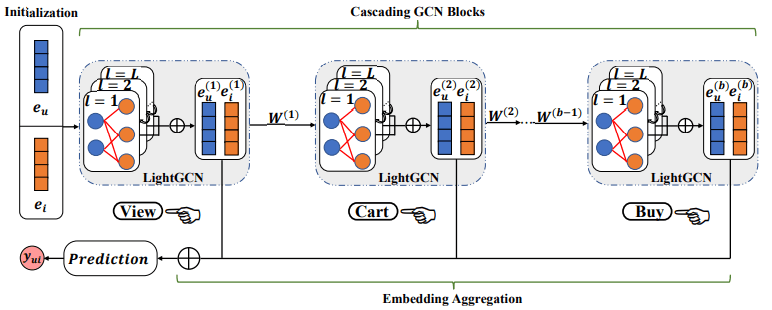
\includegraphics[width=0.9\textwidth]{images/2image7.png}
\caption{โครงสร้างสถาปัตยกรรมของโมเดล MB-CGCN แสดงการส่งต่อข้อมูลแบบลดหลั่นและการแปลงฟีเจอร์ \cite{mbcgcn_nd}}
\label{fig:mbcgcn}
\end{figure}

\subsubsection{โครงสร้างแบบบล็อกต่อเนื่อง}
ระบบแบ่งการทำงานออกเป็นบล็อกย่อยตามลำดับพฤติกรรม โดยเลือกใช้ LightGCN ที่มีความซับซ้อนน้อยแต่ประสิทธิภาพสูงเป็นแกนกลางในการประมวลผล

\subsubsection{การแปลงและคัดกรองฟีเจอร์}
จุดเด่นที่สำคัญที่สุดคือการใช้เมทริกซ์การแปลงค่า มาคั่นระหว่างบล็อกพฤติกรรม ทำหน้าที่เสมือนตัวกรอง ที่คัดแยกเฉพาะฟีเจอร์ที่มีประโยชน์ และตัดทิ้งสัญญาณรบกวน จากพฤติกรรมก่อนหน้า ไม่ให้ส่งผลเสียต่อการเรียนรู้ในขั้นถัดไป

\subsubsection{การปรับจูนด้วยพฤติกรรมเป้าหมาย}
แตกต่างจาก NMTR ที่ใช้ Multi-task learning MB-CGCN พิสูจน์ให้เห็นว่าการใช้สัญญาณสอนจากพฤติกรรมเป้าหมายเพียงอย่างเดียว จะช่วยให้โมเดลโฟกัสที่วัตถุประสงค์หลักทางธุรกิจได้อย่างแม่นยำที่สุด ในโครงงานนี้พฤติกรรมเป้าหมายตามการออกแบบคือการเช่า ผลการเปรียบเทียบประสิทธิภาพระหว่าง MB-CGCN กับโมเดลพื้นฐานแสดงในตารางที่ \ref{tab:mbcgcn_compare}
                                     
\begin{table}[H]
\centering
\caption{เปรียบเทียบประสิทธิภาพระหว่าง MB-CGCN กับโมเดลพื้นฐาน \cite{mbcgcn_nd}}
\label{tab:mbcgcn_compare}
\resizebox{\textwidth}{!}{%
\begin{tabular}{|c|c|c|c|c|c|c|c|c|c|c|c|}
\hline
\textbf{Dataset} & \textbf{Metric} & \textbf{MF-BPR} & \textbf{NeuMF} & \textbf{LightGCN} & \textbf{RGCN} & \textbf{GNMR} & \textbf{NMTR} & \textbf{MBGCN} & \textbf{CRGCN} & \textbf{MB-CGCN} & \textbf{Improv.} \\
\hline
\multirow{6}{*}{Beibei} & Recall@10 & 0.0191 & 0.0232 & 0.0391 & 0.0363 & 0.0413 & 0.0429 & 0.0470 & 0.0459 & \textbf{0.0579} & 23.2\% \\ \cline{2-12}
 & NDCG@10 & 0.0049 & 0.0135 & 0.0209 & 0.0188 & 0.0221 & 0.0198 & 0.0259 & 0.0324 & \textbf{0.0381} & 17.6\% \\ \cline{2-12}
 & Recall@20 & 0.0531 & 0.0736 & 0.0717 & 0.0684 & 0.0729 & 0.0776 & 0.0792 & 0.0891 & \textbf{0.0972} & 9.1\% \\ \cline{2-12}
 & NDCG@20 & 0.0239 & 0.0290 & 0.0270 & 0.0274 & 0.0279 & 0.0296 & 0.0330 & 0.0348 & \textbf{0.0404} & 16.1\% \\ \cline{2-12}
 & Recall@50 & 0.1014 & 0.1402 & 0.1347 & 0.1309 & 0.1391 & 0.1453 & 0.1493 & 0.1694 & \textbf{0.1924} & 13.6\% \\ \cline{2-12}
 & NDCG@50 & 0.0330 & 0.0405 & 0.0366 & 0.0371 & 0.0374 & 0.0399 & 0.0447 & 0.0487 & \textbf{0.0572} & 17.5\% \\ \hline
\multirow{6}{*}{Tmall} & Recall@10 & 0.0076 & 0.0236 & 0.0411 & 0.0215 & 0.0368 & 0.0282 & 0.0509 & 0.0855 & \textbf{0.1233} & 44.2\% \\ \cline{2-12}
 & NDCG@10 & 0.0036 & 0.0128 & 0.0240 & 0.0104 & 0.0216 & 0.0137 & 0.0294 & 0.0439 & \textbf{0.0677} & 54.2\% \\ \cline{2-12}
 & Recall@20 & 0.0244 & 0.0311 & 0.0546 & 0.0326 & 0.0608 & 0.0642 & 0.0691 & 0.1369 & \textbf{0.2007} & 46.6\% \\ \cline{2-12}
 & NDCG@20 & 0.0155 & 0.0152 & 0.0266 & 0.0125 & 0.0263 & 0.0303 & 0.0350 & 0.0676 & \textbf{0.0880} & 30.2\% \\ \cline{2-12}
 & Recall@50 & 0.0393 & 0.0494 & 0.0874 & 0.0411 & 0.0971 & 0.1034 & 0.1117 & 0.2325 & \textbf{0.3322} & 42.9\% \\ \cline{2-12}
 & NDCG@50 & 0.0197 & 0.0193 & 0.0338 & 0.0160 & 0.0336 & 0.0383 & 0.0455 & 0.0866 & \textbf{0.1134} & 30.9\% \\ \hline
\end{tabular}%
}
\end{table}

% -----------------------------------------------------------
\section{ทฤษฎีพื้นฐานของการพัฒนาเว็บแอปพลิเคชัน (Fundamentals of Web Application Development)}
% -----------------------------------------------------------
เนื่องจากโครงงานนี้เป็นส่วนหนึ่งของการพัฒนาเว็บแอปพลิเคชัน ทฤษฎีที่มาเกี่ยวข้องคือการออกแบบสถาปัตยกรรมที่สามารถเรียกใช้งานโมเดล ML ได้ \cite{sommerville2016}

\subsection{สถาปัตยกรรมสามระดับ (Three-Tier Architecture)}

รูปแบบมาตรฐานที่ช่วยให้การพัฒนาระบบเป็นระเบียบ แบ่งออกเป็น 3 ส่วนหลัก ได้แก่

\subsubsection{ส่วนแสดงผล (Presentation Tier)}
ที่ติดต่อกับผู้ใช้ ทำหน้าที่เป็นส่วนต่อประสานกับผู้ใช้ (User Interface) เพื่อรับข้อมูลและแสดงผลลัพธ์ ในโครงงานนี้พัฒนาด้วย React ซึ่งทำงานในรูปแบบ Single Page Application (SPA) เพื่อมอบประสบการณ์การใช้งานที่ลื่นไหลและตอบสนองไว

\subsubsection{ส่วนประมวลผล (Application Tier)}
ซึ่งเป็นที่อยู่ของตรรกะทางธุรกิจและระบบแนะนำ เปรียบเสมือนสมองของระบบที่มี Business Logic ในบริบทของโครงงาน AI ชั้นนี้จะทำหน้าที่เป็น ตัวกลางประสานงานที่รับคำขอจากส่วนแสดงผล และส่งต่อไปยัง Model Service ผ่าน API รวมถึงจัดการเรื่องความปลอดภัยและการตรวจสอบข้อมูล

\subsubsection{ส่วนข้อมูล (Data Tier)}
สำหรับจัดเก็บฐานข้อมูล รับผิดชอบการจัดเก็บข้อมูลให้มีความคงทน โดยเลือกใช้ PostgreSQL เป็นระบบจัดการฐานข้อมูลเพียงระบบเดียว ทั้งสำหรับข้อมูลที่มีโครงสร้างชัดเจน เช่น ข้อมูลสมาชิก มังงะ สำเนาหนังสือ ตะกร้าสินค้า และรายการเช่า รวมถึง Log พฤติกรรมของผู้ใช้ที่ใช้เป็นข้อมูลนำเข้าให้ระบบแนะนำ ซึ่งจัดเก็บในรูปแบบตารางปกติเช่นเดียวกัน การใช้ฐานข้อมูลเดียวช่วยลดความซับซ้อนของระบบ รักษาความสอดคล้องของข้อมูลผ่านความสัมพันธ์ระหว่างตาราง ง่ายต่อการดูแลรักษา และขยายระบบในอนาคต

\subsection{การทำให้ระบบแนะนำพร้อมใช้งาน (Model Deployment)}

ในขั้นตอนนี้ จะเป็นการนำโมเดล Machine Learning มาเชื่อมต่อกับเว็บแอปพลิเคชันผ่าน API โดยใช้เครื่องมืออย่าง Flask หรือ FastAPI เพื่อให้สามารถรับส่งข้อมูลผลลัพธ์ได้แบบ Real-time นอกจากนี้ การใช้เทคโนโลยี Containerization อย่าง Docker ยังเข้ามาช่วยจัดการสภาพแวดล้อมการทำงาน ลดปัญหาความขัดแย้งของซอฟต์แวร์ และทำให้การติดตั้งบนเซิร์ฟเวอร์จริงมีความเสถียรยิ่งขึ้น \cite{mltestscore_nd}